\documentclass{acm_proc_article-sp}

\usepackage{amsmath,amssymb}
\usepackage{latexsym}
\usepackage{indentfirst}
\usepackage{blindtext}
\usepackage{graphicx}
\usepackage{caption}
\usepackage{subcaption}
\usepackage{url}

\DeclareMathOperator*{\argmax}{arg\,max}
\DeclareMathOperator*{\minbelow}{min}

\begin{document}

\title{Object Tracking}
\subtitle{A Quantitative Comparison}
\numberofauthors{6}
\author{Chuhang Zou, Zheng Yan, Yi Shi, Qing Ren, Caihua Shan, Jueji Yang}
\maketitle

\begin{abstract}
Object tracking is a such import task in computer vision that many kinds of methods are devoleped to solve this problem. Most of these methods have released their codes and datasets on the Internet. It is meaningful research to evaluate these methods with unified criteria. We will briefly introduce these algorithms and use some of the datasets from Internet to test all the algorithms on some criterion about tracking window precision.
\end{abstract}

\section{Introduction}
Object tracking is one of the core problems in a wide range of applications in computer vision, such as surveillance, human computer interaction, augmented reality, and medical imaging. In most areas of computer vision like scene understanding and action recognition, object tracking is regarded as an essential component. Object tracking problem is to estimate the position of target in video sequence given the position of the target in the first frame. Most algorithms perform bad when occlusion, out-of-view appear in the sequence.

\section{Related Work}


\section{Evaluated Algorithms}

In this report, we investigate 6 visual tracking work and search for an appropriate evaluation criteria for those work. The 6 work are studied by 6 different people and each provide a report as a summary of their progress.


\subsection{Struck: Structured Output Tracking with Kernels}
This section demonstrates the tracking work by Jueji Yang.

\subsubsection{Struck}
Struck\cite{struck} is different from other tracking-by-detection algorithms. Struck learns a function that directly estimates the object transformation between frames. Discriminant function $F:\mathcal{X} \times \mathcal{Y} \to \mathcal{R}$ with $X$ the sequence of images and $Y$ the possible bounding boxes transformations is used to predict:
\[
y_t = f(x_t^{P_{t-1}}) = \argmax_{y\in \mathcal{Y}}F(x_t^{P_{t-1}},y)
\]
where $t$ is time. $x_t^{P_{t-1}}$is the image with estimated bounding box at time $t-1$ and image pixels at time $t$. $F$ measures the compatibility between $(x,y)$ pairs, when $x$ and $y$ are well matched, $F$ gives a high score:
\[
F(x,y)=\langle w, \Phi(x,y) \rangle
\]
The parameter $w$ can be optimized by:
\begin{align}
\minbelow_w	&\frac{1}{2}||w||^2 + C \sum_{i=1}^n\xi_i\nonumber\\
	s.t.	&\forall i: \xi_i \ge 0\nonumber\\
			&\forall i, \forall y\not= y_i : \langle w, \delta\Phi_i(y)\rangle \ge \Delta(y_i,y)-\xi_i
\end{align}
$\delta\Phi_i(y)=\Phi(x_i, y_i) - \Phi(x_i, y)$. This optimization aims to ensure that the value of $F(x_i, y_i)$ is greater than $F(x_i, y)$ for $y\not= y_i$. $1-\Delta(y,\bar{y})$ is the bounding box overlap between $y$ and $\bar{y}$.

The paper optimize the dual form of the optimization which will not be listed here in detail. $\Phi(x,y)$ only appears in inner products in the dual form of this optimization. So a joint kernel function $k(x,y,\bar{x},\bar{y}) = \langle \Phi(x,y), \Phi(\bar{x},\bar{y})\rangle$ is used which is the kernel between features(Haar, Histogram) of cropped boxes of images. And SMO-style step is also used to optimize the dual secondary convex optimization.

\subsection{The Deep Learning Tracker}
This section demonstrates the tracking work by Zheng Yan.

According to \cite{dlt}, they propose a novel deep learning tracker (DLT) for robust visual tracking.

During the offline training stage, they train an large stacked denoising autoencoder (SDAE) containing five small denoising autoencoders (DAEs) with the Tiny Images dataset \cite{tiny} as auxiliary image data to learn generic natural image features.
We show the architecture of DAE and the whole structure of the SDAE in Fig.~\ref{fig:dlt}(a) and Fig.~\ref{fig:dlt}(b) respectively.

During the online tracking process, an additional classification layer is added to the encoder part of the trained SDAE to result in a classification neural network.
The object to track is specified by the location of its bounding box in the first frame as a positive example.
Some negative examples are collected from the background at a short distance from the object in order to fine-tune the classification layer.
The whole network can be tuned in many times during the entire tracking process.
The overall network architecture is shown in Fig.~\ref{fig:dlt}(c).

\begin{center}
    \begin{figure}[hbt]
      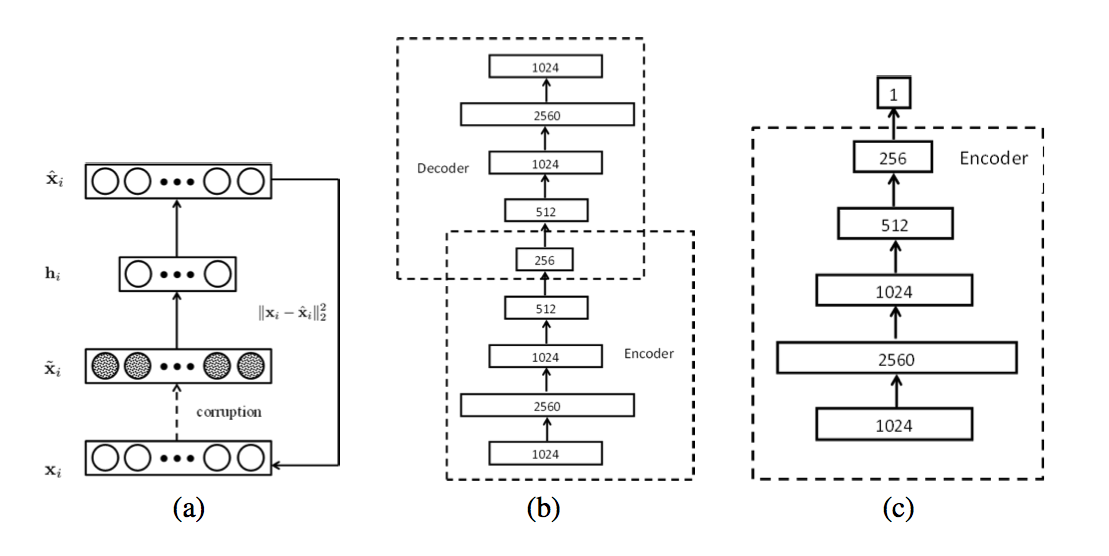
\includegraphics[width=0.5\textwidth]{dlt.png}
      \caption{Some key components of the network architecture: (a) denoising autoencoder; (b) stacked denoising autoencoder; (c) network for online tracking.}
      \label{fig:dlt}
    \end{figure}
\end{center}

\subsection{Context Tracker: Exploring Supporters and Distracters in Unconstrained Environments}
This section demonstrates the tracking work by Caihua Shan.

\subsubsection{Introduction}
    This paper uses additional context information to build a strong model. It uses two different terms: 1) Distracters are regions that have similar appearance as the target, 2) Supporters are local key-points around the object having motion correlation with the target in a short time span. The goal of this algorithm is to find all possible regions which look similar to the target to prevent drift, and to look for useful information around the target to have strong verification.
    
\subsubsection{Algorithm}
    The paper uses P-N Tracker as the basic target tracker with several extensions. It extends the randomized ferns to accept multiple objects, applies 6bitBP which helps to boost up the speed of the detector and uses online template-based object model by constructing it in binary search tree using k-means.
    \newline
    As for distracters, a testing sample confidence score is computed using Normalized Cross-Correlation(NCC) between it and the closest image patch in the object model. It chooses the best candidate as the tracking result and the remaining regions trigger new distracter trackers.
    \newline
    Assuming that there are the valid target at frame t, the supporters are extracted around the location of that target with a radius R.
    \newline
    In unconstrained environments, the target may leave the FoV, or be completely occluded by other objects. The common trackers will simply switch to another region satisfying the threshold. Here, this tracker automatically exploits all the distracters and pays attention to them by tracking them simultaneously. Also, this tracker discovers a set of supporters to robustly identify the target among other similar regions.

\subsection{Visual Tracking via Adaptive Structural Local Sparse Appearance Model}
This section demonstrates the tracking work by Yi Shi.

\subsubsection{Introduction}
Visual Tracking via Adaptive Structural Local Sparse Appearance Model (ASLA) is one of Posters in CVPR2012 and performs favorably against several state-of-the-art methods on benchmark challenge.

ASLA is an efficient methods combined with structural local sparse model and adaptive template update strategy. It samples overlapped local image patches within the target region, whose sparse coding obtained by a novel alignment-pooling method contains both spatial and partial information of the target object. This representation guarantees more accurately location and less occlusion drift. In addition, the online adaptive template strategy based on both incremental subspace learning and sparse representation is employed in coding, far more improving the performance compared by methods based on static local or holistic sparse dictionary when there is similar object in the scenes.

\subsubsection{Algorithm}
The proposed algorithm is implemented in MATLAB and runs at 1.5 frames per second on a Pentium 2.7 GHz Dual Core PC with 2GB memory.

The $l_1$ minimization problem is solved with the SPAMS package and the regularization constant $\lambda$ is set to 0.01 in all experiments. For each sequence, the location of the target object is manually labeled in the first frame. We resize the target image patch to $32\times 32$ pixels and extract overlapped $16\times16$ local patches within the target region with 8 pixels as step length. As for the template update, 8 eigenvectors are used to carry out incremental subspace learning method in all experiments every 5 frames.

\subsection{Context Tracker: Exploring Supporters and Distracters in Unconstrained Environments}
This section demonstrates the tracking work by Qing Ren.

\subsubsection{Introduction}
Tracking is a fundamental problem in computer vision, sometimes it is desirable to track an object with little prior knowledge. Almost all the methods by Tracking-by-detection, a extremely useful approach, have one thing in common, that is a sparse sampling strategy. Several samples, near the target, will be collected in every frame. For each sample, it typically characterizes a subwindow the same size as the target and most of the samples have a huge amount of overlap, causing a lot of redundancy. In order to overcome this weakness, we address a new theory. We show that the process of taking subwindows of an image indce circulant structure. Then establishing links to Fourier analysis that allows the use of the Fast Fourier Transform to quickly incorporate information from all subwindows, without iterating over them. Classification on non-linear feature spaces with the Kernel Trick can be done as efficiently as in the original image space. All running in $O(n^2 logn)$ for $n * n$ images.


\subsection{Discrete-Continuous Optimization for Multi-Target Tracking}
This section demonstrates the tracking work by Chuhang Zou.

\subsubsection{Introduction}
Recent approaches for multi-target tracking often use discrete optimization. However, this has the disadvantage that trajectories need to be pre-computed or represented discretely, thus limiting accuracy. In this paper, the author instead formulate multi-target tracking as a discrete-continuous optimization problem that handles each aspect in its natural domain and allows leveraging powerful methods for multi-model fitting. Data association is performed using discrete optimization with label costs, yielding near optimality. Trajectory estimation is posed as a continuous fitting problem with a simple closed-form solution, which is used in turn to update the label costs.

\subsubsection{Algorithm}
Targets are separated from the background in a preprocessing step and form a set of target hypotheses, which are then used to infer the targets¡¯ trajectories. Then algorithm then run a sliding window detector, based on SVM classification of histograms of oriented gradients (HOG) and relative optical flow (HOF). The detector yields a set of target hypotheses D.

Given the set of target hypotheses D, the goal is to identify a set of target trajectories $\tau = {\tau_1,\ldots,\tau_N}$. This implies that it also need to search for a data association $f$, which for each detection $d \in D$ assigns a label $f_f \in L = {1,\ldots,N}\bigcup \emptyset$. Thereby a detection is either identified as belonging to one of the trajectories or, using the additional outlier label $\emptyset$, identified as a false alarm.
The eventual aim is to perform multi-target tracking by minimizing a joint energy $E(\tau , f)$ w.r.t. the trajectories $\tau$ and the data association $f$. 

\section{Experiments}
We choose ten image sequences from benchmark website\cite{dataset}. We use success rate score = area($R_T \bigcap R_G$)$/$area($R_T \bigcup R_G$) which is described both in Section ~\ref{sec:asla_section} and others tests\cite{benchmark}. And then calculate the percentage of frames that has a score bigger than Overlap threshold showed in Fig.~\ref{fig:soccer}.

\begin{figure}[hbt]
    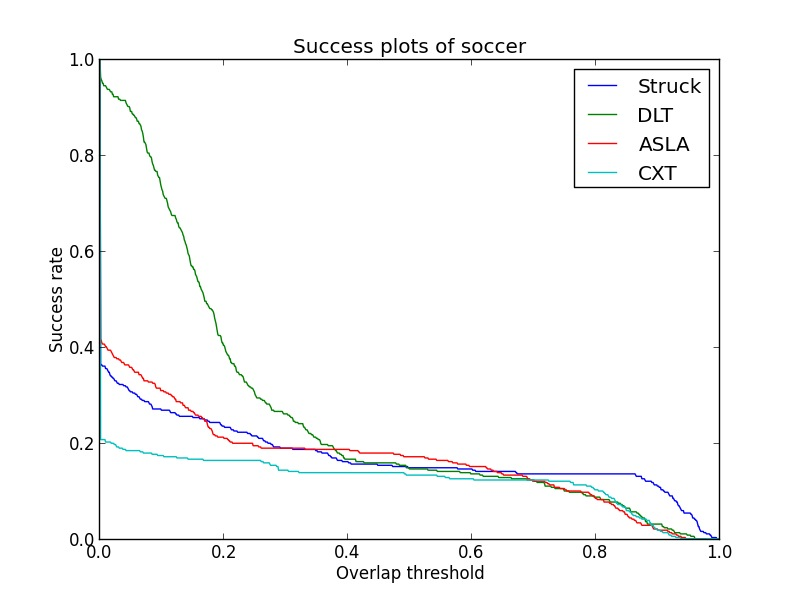
\includegraphics[width=200pt]{soccer.jpg}
    \caption{success rate score plot of soccer sequences}
    \label{fig:soccer}
\end{figure}

\begin{figure}[hbt]
    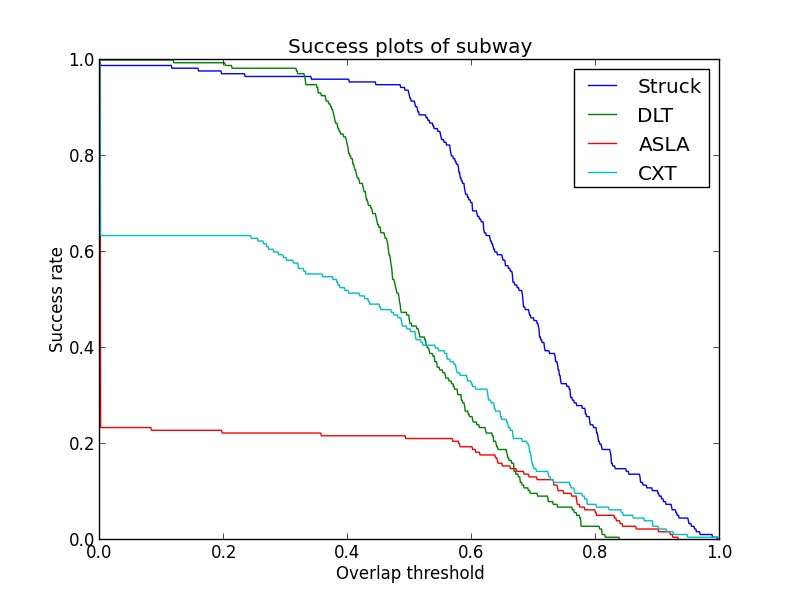
\includegraphics[width=200pt]{subway.jpg}
    \caption{success rate score plot of subway sequences}
    \label{fig:subway}
\end{figure}

\begin{figure}[hbt]
    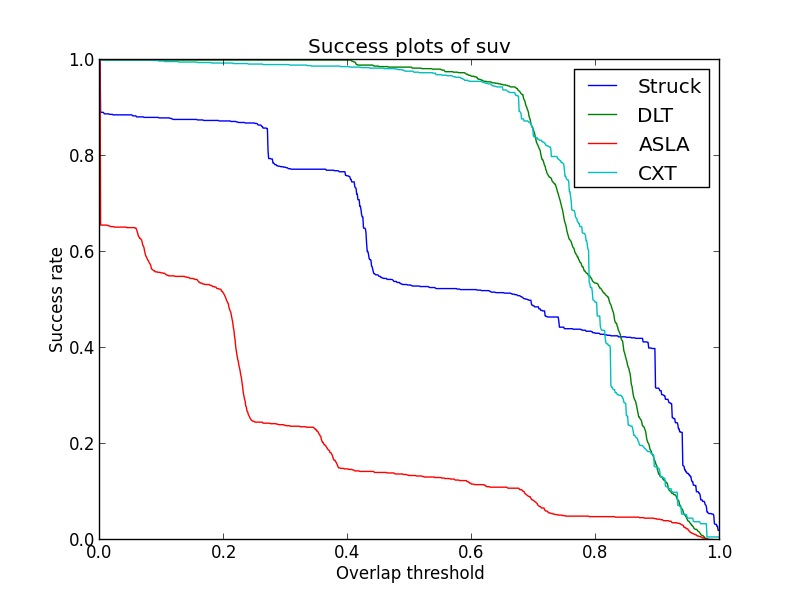
\includegraphics[width=200pt]{suv.jpg}
    \caption{success rate score plot of suv sequences}
    \label{fig:suv}
\end{figure}

\begin{figure}[hbt]
    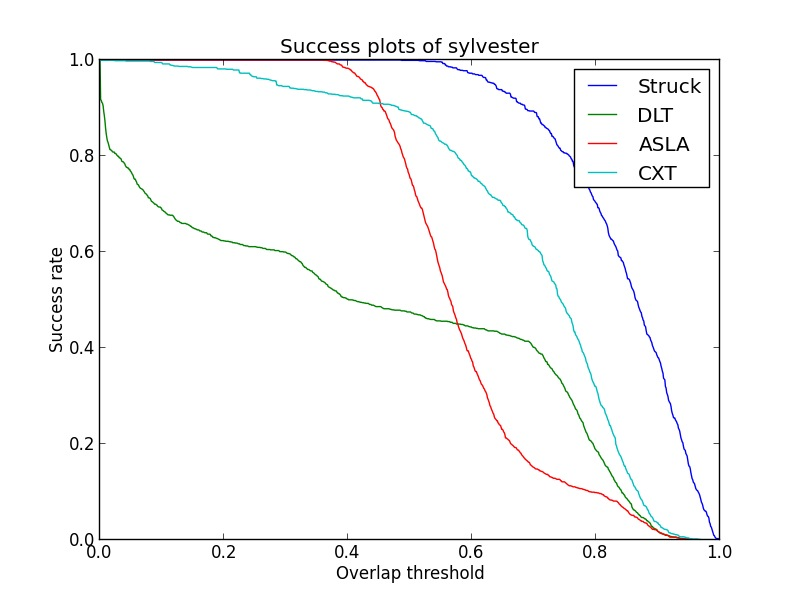
\includegraphics[width=200pt]{sylvester.jpg}
    \caption{success rate score plot of sylvester sequences}
    \label{fig:sylvester}
\end{figure}

\begin{figure}[hbt]
    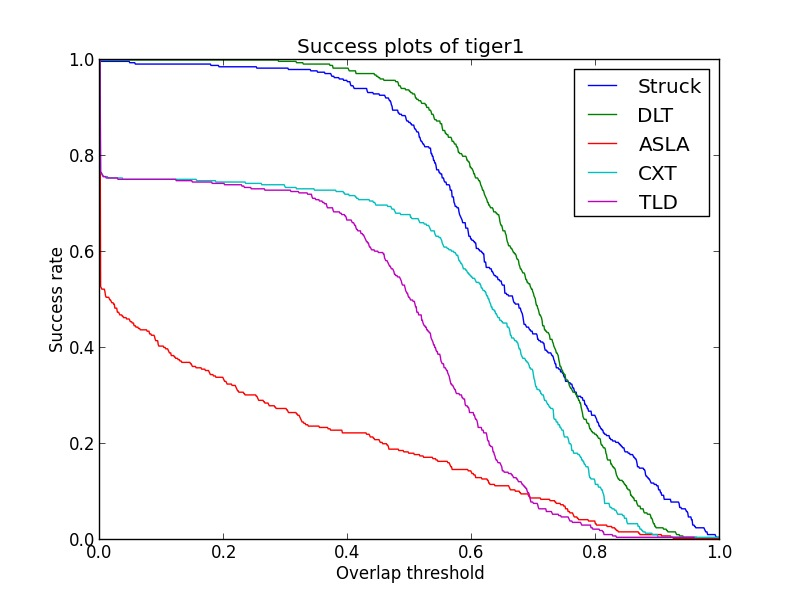
\includegraphics[width=200pt]{tiger1.jpg}
    \caption{success rate score plot of tiger1 sequences}
    \label{fig:tiger1}
\end{figure}

\begin{figure}[hbt]
    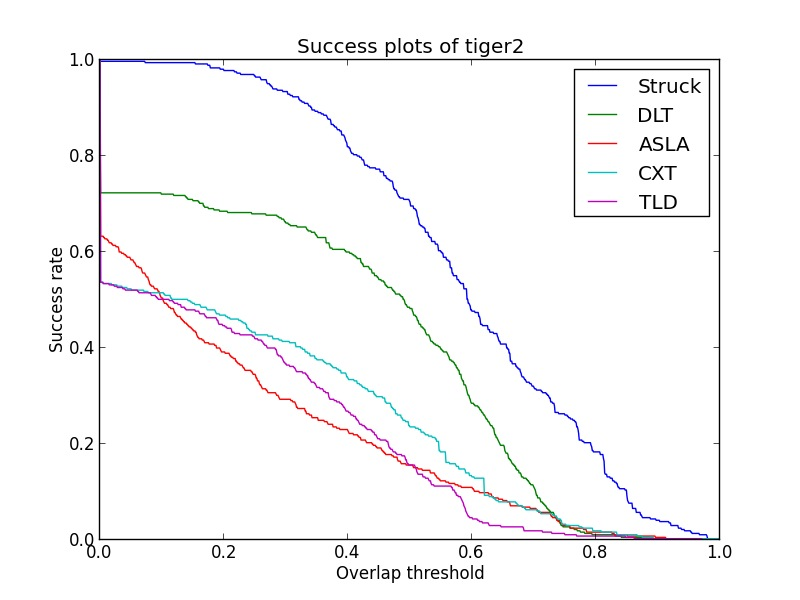
\includegraphics[width=200pt]{tiger2.jpg}
    \caption{success rate score plot of tiger2 sequences}
    \label{fig:tiger2}
\end{figure}

\begin{figure}[hbt]
    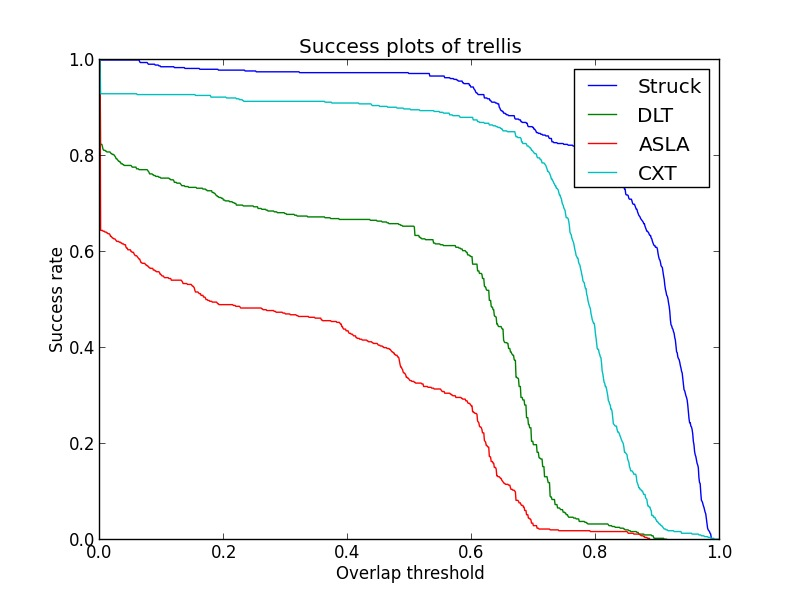
\includegraphics[width=200pt]{trellis.jpg}
    \caption{success rate score plot of trellis sequences}
    \label{fig:trellis}
\end{figure}

\begin{figure}[hbt]
    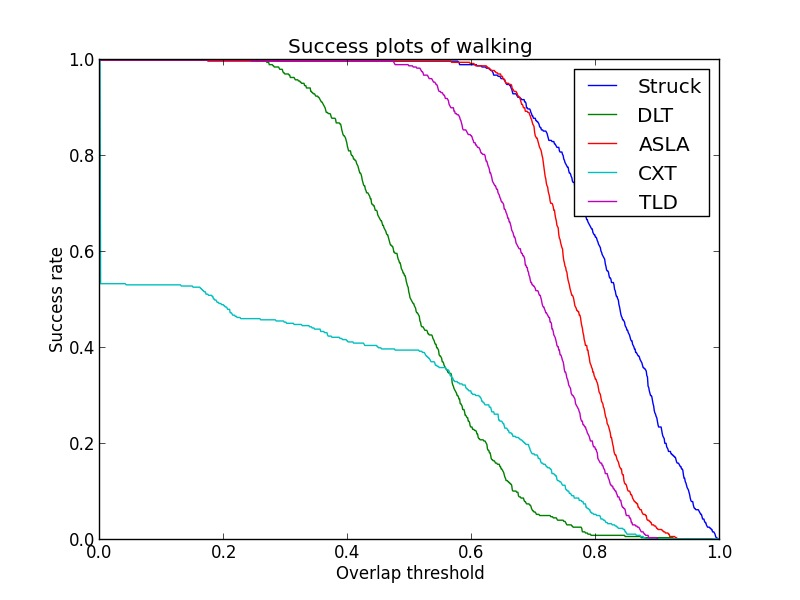
\includegraphics[width=200pt]{walking.jpg}
    \caption{success rate score plot of walking sequences}
    \label{fig:walking}
\end{figure}

\begin{figure}[hbt]
    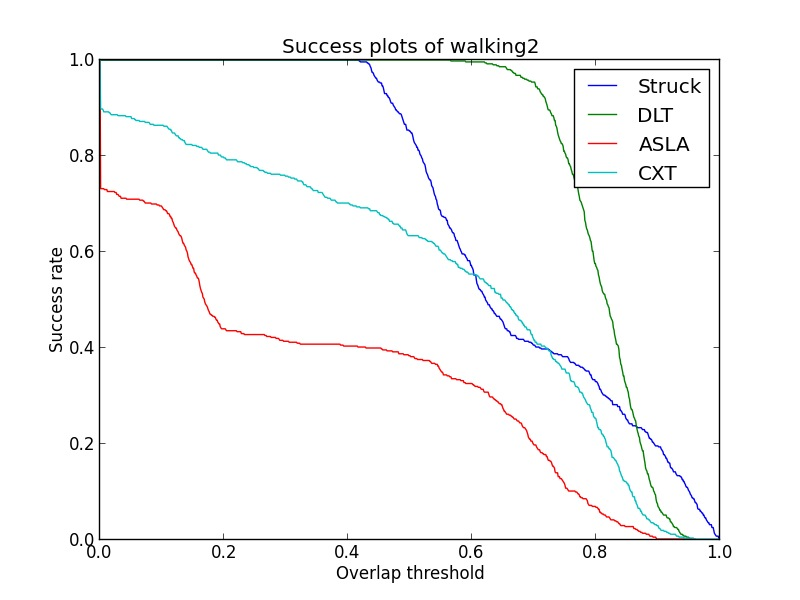
\includegraphics[width=200pt]{walking2.jpg}
    \caption{success rate score plot of walking2 sequences}
    \label{fig:walking2}
\end{figure}

\begin{figure}[hbt]
  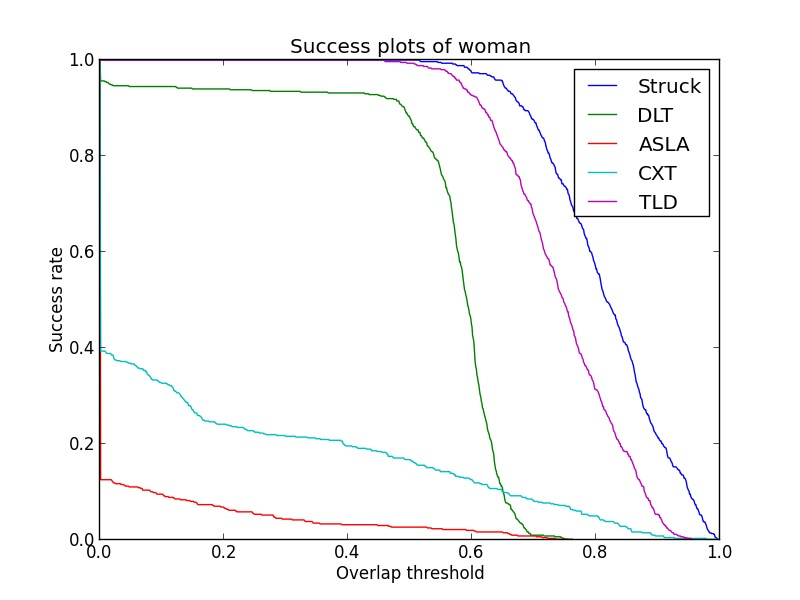
\includegraphics[width=200pt]{woman.jpg}
  \caption{success rate score plot of woman sequences}
  \label{fig:woman}
\end{figure}

Struck detects 9 frames per second with budget size of 100 and Haar feature. In these ten image sequence, truck performs not good in Soccer and SUV. Soccer image has many pieces of ribbons which has stronger effect on Haar feature than human faces. In SUV image, the SUV is occluded by trees and traffic lights, histogram of color feature is litter better than the Haar feature.

DLT detects 4~5 frames per second. In the tiger1 and tiger2 sequence, the target is a fast moving tool with motion blur. DLT with a higher value of x and y translation can track tiger1 successfully, while lost track of tiger2 in about frame 160. In the woman sequence, the woman is severely occluded several times by the parked cars. DLT tracker fails when the woman walks close to the car at about frame 130.

In the Woman, Walking, Walking2 and Subway sequence, the target is obstructed by moving or feature-similar objects, ASLA performs bad in this sequence. In the Sylvester sequence,the target is moving with illumination varying, ASLA does well in this sequence. In other sequence, it got lost in some frames but follows almost frames overall. From another respective,  though the tracker follows the target, the areas it predict has deviation compared with ground truth.

\begin{table}
	\centering
	\begin{tabular}{|c|c|l|} \hline
		Method & FPS\\ \hline
		Struck & 15.8\\ \hline
		DLT & 17.5\\ \hline
		CXT & 15.3\\ \hline
		ASLA & 8.5\\ \hline
		Zou & ?.?\\ \hline
		CSK & ?.?\\ \hline
	\end{tabular}
	\caption{Comparison of average running time on woman video sequences (in fps).}
\end{table}


\section{Conclusions}
This paragraph will end the body of this sample document.
Remember that you might still have Acknowledgments or
Appendices; brief samples of these
follow.  There is still the Bibliography to deal with; and
we will make a disclaimer about that here: with the exception
of the reference to the \LaTeX\ book, the citations in
this paper are to articles which have nothing to
do with the present subject and are used as
examples only.


\begin{thebibliography}{99}
\bibitem{struck}
S. Hare, A. Saffari, and P. H. S. Torr. Struck: Structured Output Tracking with Kernels. In ICCV, 2011.

\bibitem{shi1}
A. Adam, E. Rivlin, and I. Shimshoni. Robust fragments-based tracking using the integral histogram. In CVPR, 2006.

\bibitem{shi2}
B. Babenko, M.-H. Yang, and S. Belongie. Visual tracking with online multiple instance learning. In CVPR, 2009.

\bibitem{shi3}
J. Kwon and K. M. Lee. Visual tracking decomposition. In CVPR, 2010.

\bibitem{shi4}
D. Ross, J. Lim, R.-S. Lin, and M.-H. Yang. Incremental learning for robust visual tracking. IJCV, 77(1): 125141, 2008.

\bibitem{shi5}
J. Santner, C. Leistner, A. Saffari, T. Pock, and H. Bischof. Prost: Parallel robust online simple tracking. In CVPR, 2010.

\bibitem{shi6}
X. Mei and H. Ling. Robust visual tracking using L1 minimization. In ICCV, 2009.

\bibitem{shi7}
Z. Kalal, J. Matas, and K. Mikolajczyk. P-N learning: Bootstrapping binary classifiers by structural constraints. In CVPR, 2010.

\bibitem{dlt}
Wang, Naiyan, and Dit-Yan Yeung. Learning a Deep Compact Image Representation for Visual Tracking. Advances in Neural Information Processing Systems. 2013.

\bibitem{tiny}
Torralba, Antonio, Robert Fergus, and William T. Freeman. 80 million tiny images: A large data set for nonparametric object and scene recognition. Pattern Analysis and Machine Intelligence, IEEE Transactions on 30.11 (2008): 1958-1970.

\bibitem{benchmark}
Y.Wu, J. Lim, M.H. Y. Online Object Tracking: A Benchmark. In CVPR, 2013

\bibitem{dataset}
\url{https://sites.google.com/site/trackerbenchmark/benchmarks/v10}

\end{thebibliography}

\end{document}
